\documentclass[amssymb,amsmath]{beamer}
\usetheme{Boadilla}
%\usepackage[english]{babel}
\usepackage{graphicx}
\usepackage{wrapfig}
\usepackage{color}
\usepackage{multicol}
\usepackage{tikz}
%%%%%%%%%%%%%%%
\usepackage{bookmath} % definitions and shortcuts
\bibliographystyle{apsrev}
%%%%%%%%%%%%%%%
\setbeamertemplate{frametitle}{ \bf
\begin{centering} 
\insertframetitle 
\par 
\end{centering} 
}
%%%%%%%%%%%%%%%% 
\newcommand{\black}{\textcolor{black}}
\newcommand{\blue}{\textcolor{blue}}
\newcommand{\red}{\textcolor{red}}
\newcommand{\green}{\textcolor{green}}
\newcommand{\olive}{\textcolor{olive}}
\newcommand\Fontvi{\fontsize{9}{9}\selectfont}
\newcommand\Fontvii{\fontsize{4}{4}\selectfont}
\newcommand\Fontv{\fontsize{11}{11}\selectfont}
\newcommand\Fontb{\fontsize{15}{15}\selectfont}
\newcommand\Fontsm{\fontsize{13}{13}\selectfont}
%%%%%%%%%%%%%%%%%%%%%%%%%%%%%%%%%%%%%%%%%%%%%%%%%%%%%%%
%%%%%%%%%%%%%%%%%%%%%%%%%%%%%%%%%%%%%%%%%%%%%%%%%%%%%%%

\title[]{High Temperature Superconductivity in Hydrides}
\author[brosemeyer@physics.montana.edu]{Ben Rosemeyer \\ \small Advisor: Anton Vorontsov}
\institute[MSU]{

\includegraphics[scale=0.2]{./figures/MSUlogo.jpg}\\[0.5cm]
Condensed Matter Seminar
}

\date[CMP Nov 30 2015]{\small\today}



\begin{document}
\frame{\titlepage}
%%%%%%%%%%%%%%%%%%%%%%%%%%%
\tikzstyle{every picture}+=[remember picture]
%%%%%%%%%%%%%%%%%%%%%%%%%%%
%\section*{Outline}
%\frame{\tableofcontents}
\begin{frame}
\frametitle{OUTLINE}
\begin{block}{}
-New $T_c$ record in Sulfur Hydride system at extreme pressure\\ 
\quad $T_c \approx 200K$, $P\approx 150GPa$ (Drozdov et al, Nature 2015)
\end{block}\centering
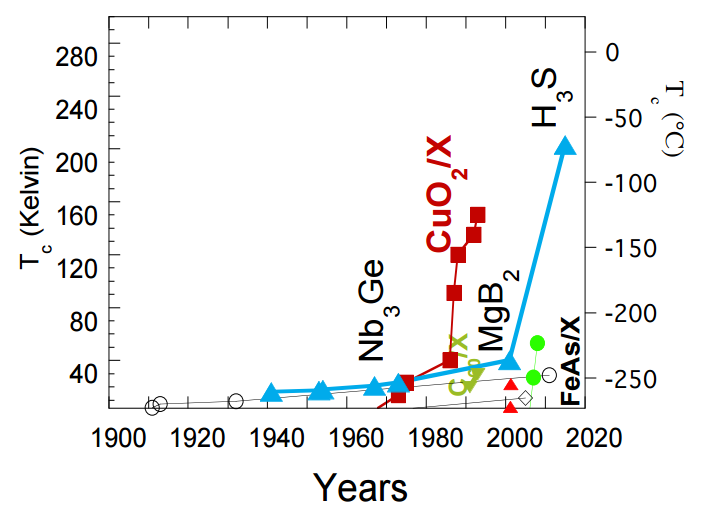
\includegraphics[scale=0.25]{./figures/Tc_vs_year.png} \\
\begin{block}{\red{THEORETICAL NEEDS}}
-Describe P-T phases and transitions of metallization (Enthalpy) \\
-Find electron and phonon dispersions (Density of States \\
-Develop $T_c$ calculation (Eliashberg,  McMillan-Dynes-Allen)
\end{block}
\end{frame}
%%%%%%%%%%%%%%%%%%%%%%%%%%%%%%%%%%%%%%%%%%%%%%%%%%%%%%%%%%%%%%%%%%%%%%%%%%%%%%%%%%%%%%%%%%%%%%%%%%%%%%%%%%%%%%%%%%%%%%%%%%%%
%%%%%%%%%%%%%%%%%%%%%%%%%%%%%%%%%%%%%%%%%%%%%%%%%%%%%%%%%%%%%%%%%%%%%%%%%%%%%%%%%%%%%%%%%%%%%%%%%%%%%%%%%%%%%%%%%%%%%%%%%%%%
%%%%%%%%%%%%%%%%%%%%%%%%%%%%%%%%%%%%%%%%%%%%%%%%%%%%%%%%%%%%%%%%%%%%%%%%%%%%%%%%%%%%%%%%%%%%%%%%%%%%%%%%%%%%%%%%%%%%%%%%%%%%
\begin{frame}
\frametitle{BACKGROUND}
\begin{block}{High $T_c$}
Metallic Hydrogen: A High-Temperature Superconductor? \\
\quad N. W. Ashcroft, Phys. Rev. Lett. 21, 1748 (1968)\\[0.5cm]
Hydrogen Dominant Metallic Alloys: High Temperature Superconductors? \\
\quad N. W. Ashcroft, Phys. Rev. Lett. 92, 187002 (2004)
\end{block}
\begin{block}{$H_2 S$}
"No experimental studies of hydrogen sulphide are known above 100 GPa" \\
\quad Drozdov et al, Nature 2015 \\ [0.5cm]
"Metallization and superconductivity in sulfur hydride occur at such
high pressure when nothing is known in advance regarding the basic physical properties of the material
under study. Not even the chemical formula is known and it is for theory to establish, in the first place,
the very composition of the compound under investigation at such pressure." \\
\quad Gor’kov, Kresin, arXiv:1511.06926
\end{block}
\end{frame}
%%%%%%%%%%%%%%%%%%%%%%%%%%%%%%%%%%%%%%%%%%%%%%%%%%%%%%%%%%%%%%%%%%%%%%%%%%%%%%%%%%%%%%%%%%%%%%%%%%%%%%%%%%%%%%%%%%%%%%%%%%%%
%%%%%%%%%%%%%%%%%%%%%%%%%%%%%%%%%%%%%%%%%%%%%%%%%%%%%%%%%%%%%%%%%%%%%%%%%%%%%%%%%%%%%%%%%%%%%%%%%%%%%%%%%%%%%%%%%%%%%%%%%%%%
%%%%%%%%%%%%%%%%%%%%%%%%%%%%%%%%%%%%%%%%%%%%%%%%%%%%%%%%%%%%%%%%%%%%%%%%%%%%%%%%%%%%%%%%%%%%%%%%%%%%%%%%%%%%%%%%%%%%%%%%%%%%
\begin{frame}
\frametitle{EXPERIMENT}
Confirmed by \red{TWO} groups, Drozdov et al and Einaga et al, arXiv:1509.03156 \\
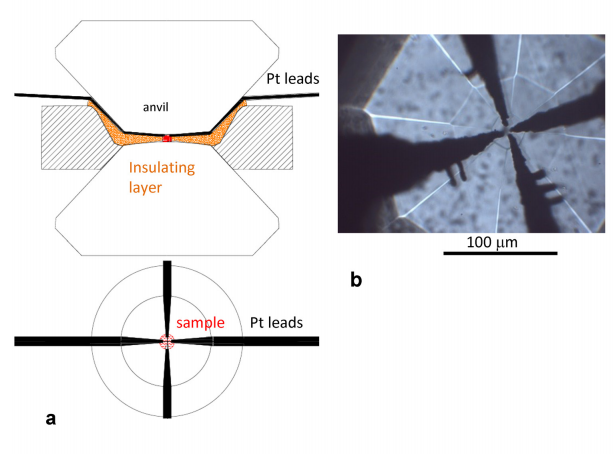
\includegraphics[scale=0.25]{./figures/diamond_anvil.png} 
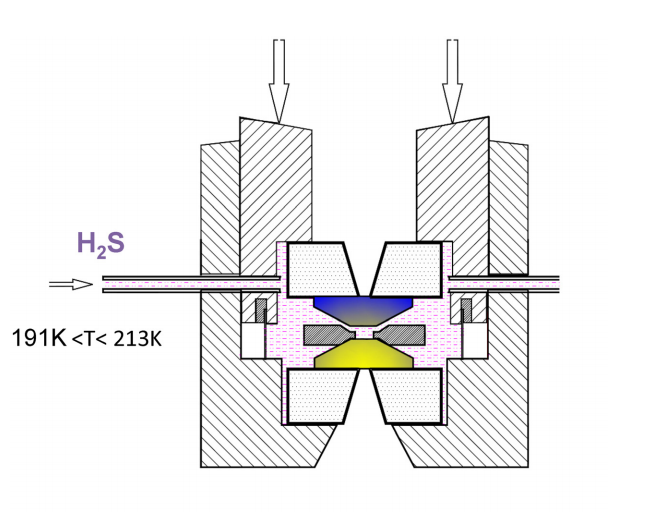
\includegraphics[scale=0.25]{./figures/diamond_anvil_fill.png} \\
Drozdov et al, Nature 2015 \\
https://vimeo.com/131914556
\end{frame}
%%%%%%%%%%%%%%%%%%%%%%%%%%%%%%%%%%%%%%%%%%%%%%%%%%%%%%%%%%%%%%%%%%%%%%%%%%%%%%%%%%%%%%%%%%%%%%%%%%%%%%%%%%%%%%%%%%%%%%%%%%%%
%%%%%%%%%%%%%%%%%%%%%%%%%%%%%%%%%%%%%%%%%%%%%%%%%%%%%%%%%%%%%%%%%%%%%%%%%%%%%%%%%%%%%%%%%%%%%%%%%%%%%%%%%%%%%%%%%%%%%%%%%%%%
%%%%%%%%%%%%%%%%%%%%%%%%%%%%%%%%%%%%%%%%%%%%%%%%%%%%%%%%%%%%%%%%%%%%%%%%%%%%%%%%%%%%%%%%%%%%%%%%%%%%%%%%%%%%%%%%%%%%%%%%%%%%
\begin{frame}
\frametitle{RESISTIVITY and ISOTOPE EFFECT}
\centering
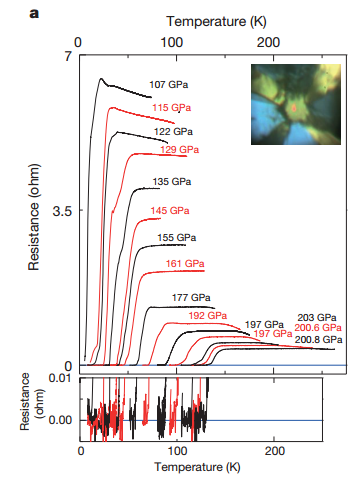
\includegraphics[scale=0.3]{./figures/resistivity_drozdov.png} 
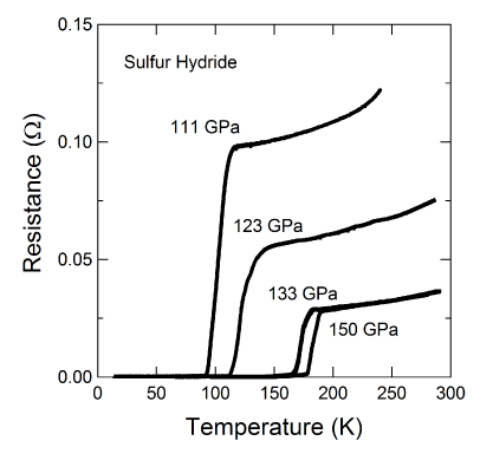
\includegraphics[scale=0.3]{./figures/resistivity_einaga.png}
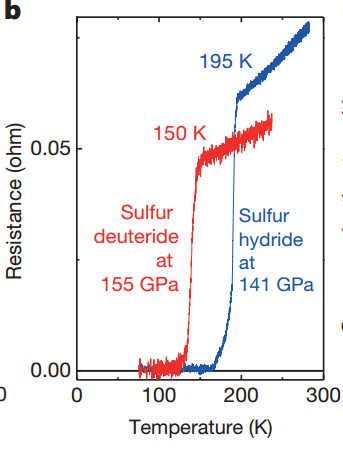
\includegraphics[scale=0.3]{./figures/isotope_drozdov.png}\\
Drozdov, Eigana, Drozdov \\

-Annealing sample resulted in higher $T_c$ and more stable measurements \\

\end{frame}
%%%%%%%%%%%%%%%%%%%%%%%%%%%%%%%%%%%%%%%%%%%%%%%%%%%%%%%%%%%%%%%%%%%%%%%%%%%%%%%%%%%%%%%%%%%%%%%%%%%%%%%%%%%%%%%%%%%%%%%%%%%%
%%%%%%%%%%%%%%%%%%%%%%%%%%%%%%%%%%%%%%%%%%%%%%%%%%%%%%%%%%%%%%%%%%%%%%%%%%%%%%%%%%%%%%%%%%%%%%%%%%%%%%%%%%%%%%%%%%%%%%%%%%%%
%%%%%%%%%%%%%%%%%%%%%%%%%%%%%%%%%%%%%%%%%%%%%%%%%%%%%%%%%%%%%%%%%%%%%%%%%%%%%%%%%%%%%%%%%%%%%%%%%%%%%%%%%%%%%%%%%%%%%%%%%%%%
\begin{frame}
\frametitle{CRITICAL TEMPERATURE}
\centering

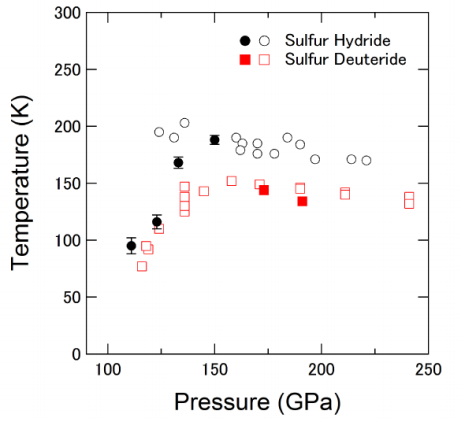
\includegraphics[scale=0.3]{./figures/PT_einaga.png}
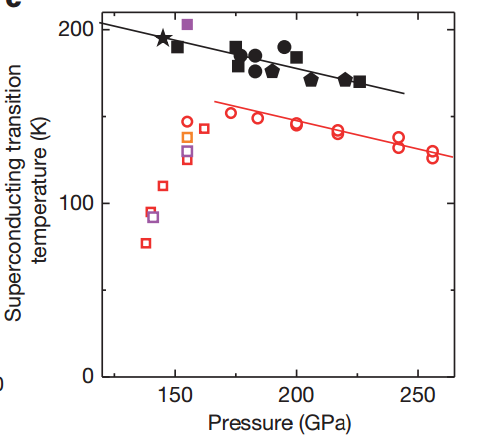
\includegraphics[scale=0.3]{./figures/PT_drozdov.png}\\
Eigana, Drozdov \\[1cm]
$T_c=10-25K$ ($P=100-250GPa$) for elemental Sulfur  
\end{frame}
%%%%%%%%%%%%%%%%%%%%%%%%%%%%%%%%%%%%%%%%%%%%%%%%%%%%%%%%%%%%%%%%%%%%%%%%%%%%%%%%%%%%%%%%%%%%%%%%%%%%%%%%%%%%%%%%%%%%%%%%%%%%
%%%%%%%%%%%%%%%%%%%%%%%%%%%%%%%%%%%%%%%%%%%%%%%%%%%%%%%%%%%%%%%%%%%%%%%%%%%%%%%%%%%%%%%%%%%%%%%%%%%%%%%%%%%%%%%%%%%%%%%%%%%%
%%%%%%%%%%%%%%%%%%%%%%%%%%%%%%%%%%%%%%%%%%%%%%%%%%%%%%%%%%%%%%%%%%%%%%%%%%%%%%%%%%%%%%%%%%%%%%%%%%%%%%%%%%%%%%%%%%%%%%%%%%%%
\begin{frame}
\frametitle{$H_2S$ DECOMPOSITION}
\centering
%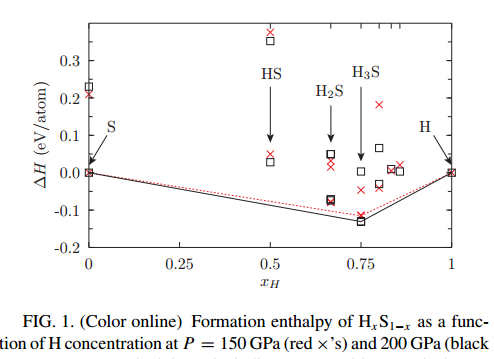
\includegraphics[scale=0.3]{./figures/decomposition_bernstein.png}
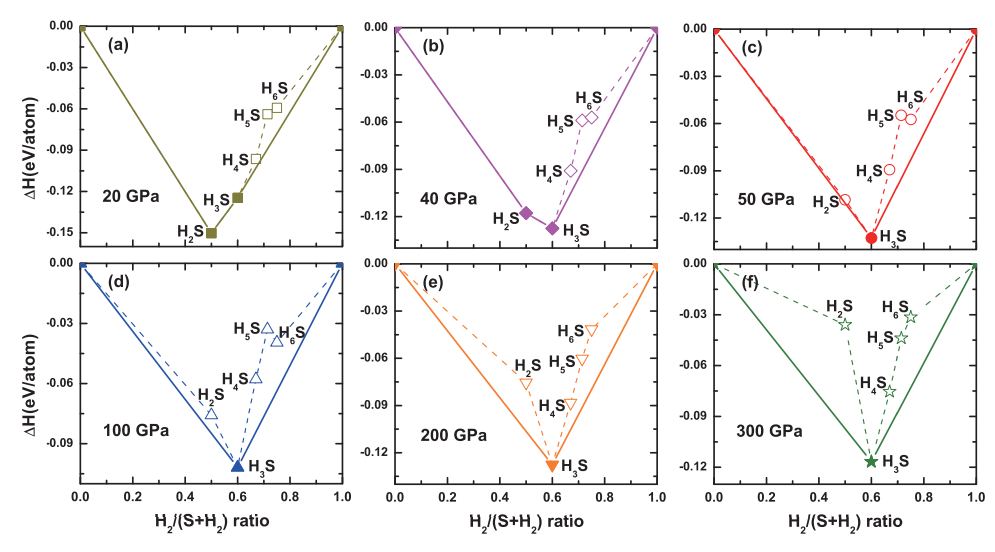
\includegraphics[scale=0.3]{./figures/decomposition_duan.png}\\
Duan et al, Scientific Reports 4, Article number: 6968 (2014)
%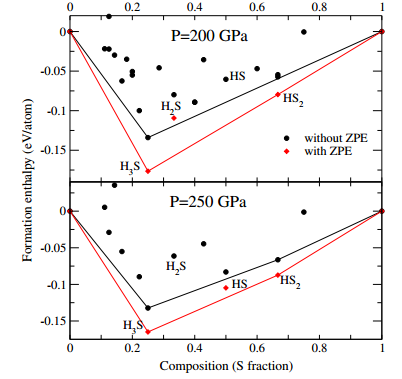
\includegraphics[scale=0.3]{./figures/decomposition_errea.png}

\begin{block}{}
$3H_2S\rightarrow 2H_3S+S$
\end{block}
\end{frame}
%%%%%%%%%%%%%%%%%%%%%%%%%%%%%%%%%%%%%%%%%%%%%%%%%%%%%%%%%%%%%%%%%%%%%%%%%%%%%%%%%%%%%%%%%%%%%%%%%%%%%%%%%%%%%%%%%%%%%%%%%%%%
%%%%%%%%%%%%%%%%%%%%%%%%%%%%%%%%%%%%%%%%%%%%%%%%%%%%%%%%%%%%%%%%%%%%%%%%%%%%%%%%%%%%%%%%%%%%%%%%%%%%%%%%%%%%%%%%%%%%%%%%%%%%
%%%%%%%%%%%%%%%%%%%%%%%%%%%%%%%%%%%%%%%%%%%%%%%%%%%%%%%%%%%%%%%%%%%%%%%%%%%%%%%%%%%%%%%%%%%%%%%%%%%%%%%%%%%%%%%%%%%%%%%%%%%%
\begin{frame}
\frametitle{METALLIZATION}
\begin{columns}\begin{column}{0.5\textwidth}
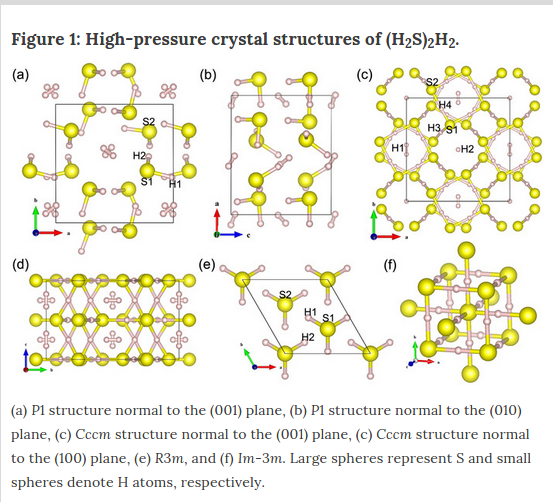
\includegraphics[scale=0.3]{./figures/structures_duan.png} \\
Duan\\[1cm]
\hspace{1cm} Flores et al, arXiv:1501.06336
\end{column}
\begin{column}{0.5\textwidth}
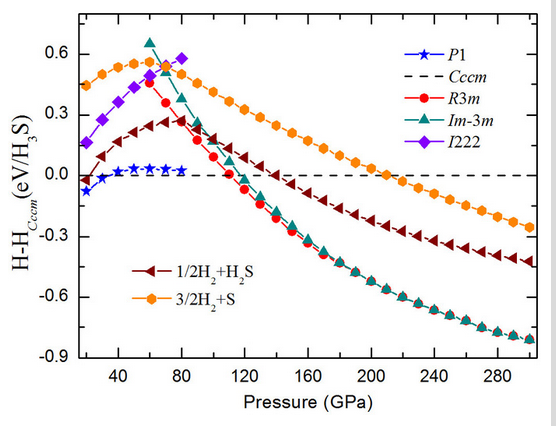
\includegraphics[scale=0.27]{./figures/enthalpy_duan.png} Duan\\
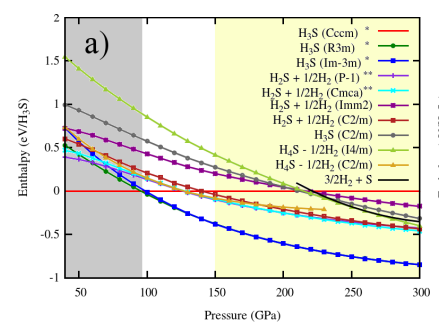
\includegraphics[scale=0.4]{./figures/enthalpy_flores.png}
\end{column}\end{columns}
\end{frame}
%%%%%%%%%%%%%%%%%%%%%%%%%%%%%%%%%%%%%%%%%%%%%%%%%%%%%%%%%%%%%%%%%%%%%%%%%%%%%%%%%%%%%%%%%%%%%%%%%%%%%%%%%%%%%%%%%%%%%%%%%%%%
%%%%%%%%%%%%%%%%%%%%%%%%%%%%%%%%%%%%%%%%%%%%%%%%%%%%%%%%%%%%%%%%%%%%%%%%%%%%%%%%%%%%%%%%%%%%%%%%%%%%%%%%%%%%%%%%%%%%%%%%%%%%
%%%%%%%%%%%%%%%%%%%%%%%%%%%%%%%%%%%%%%%%%%%%%%%%%%%%%%%%%%%%%%%%%%%%%%%%%%%%%%%%%%%%%%%%%%%%%%%%%%%%%%%%%%%%%%%%%%%%%%%%%%%%
\begin{frame}
\frametitle{METALLIZATION}
\begin{columns}\begin{column}{0.5\textwidth}
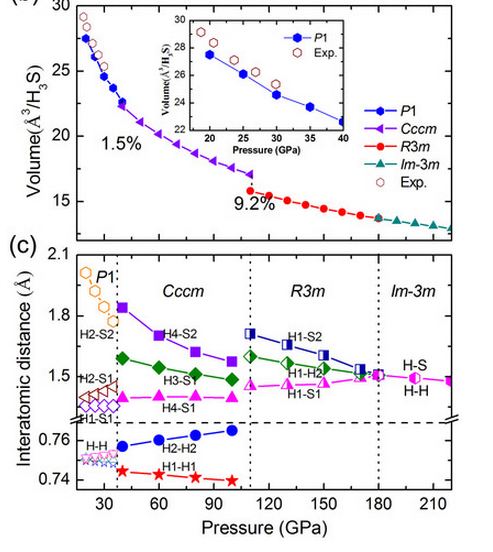
\includegraphics[scale=0.39]{./figures/transitions_flores.png}\\
-Flores
\end{column}
\begin{column}{0.45\textwidth}
General picture of phase transitions $P1\rightarrow Cccm\rightarrow R3m\rightarrow Im-3m$ is unified among theories and agrees with XRD data (Eigana), but order of  $R3m\rightarrow Im-3m$ is still under debate (See Gorkov paper)
\end{column}\end{columns}
\end{frame}
%%%%%%%%%%%%%%%%%%%%%%%%%%%%%%%%%%%%%%%%%%%%%%%%%%%%%%%%%%%%%%%%%%%%%%%%%%%%%%%%%%%%%%%%%%%%%%%%%%%%%%%%%%%%%%%%%%%%%%%%%%%%
%%%%%%%%%%%%%%%%%%%%%%%%%%%%%%%%%%%%%%%%%%%%%%%%%%%%%%%%%%%%%%%%%%%%%%%%%%%%%%%%%%%%%%%%%%%%%%%%%%%%%%%%%%%%%%%%%%%%%%%%%%%%
%%%%%%%%%%%%%%%%%%%%%%%%%%%%%%%%%%%%%%%%%%%%%%%%%%%%%%%%%%%%%%%%%%%%%%%%%%%%%%%%%%%%%%%%%%%%%%%%%%%%%%%%%%%%%%%%%%%%%%%%%%%%
\begin{frame}
\frametitle{$T_c$ CALCULATION}
Allen and Dynes Phys. Rev. B 12, 905 (1975) \\
-Using an Einstein phonon spectrum $T_c$ has \emph{Lower} bound
$T_c> \frac{\omega_E}{2\pi}\sqrt{\frac{\lambda}{1+2\mu^*}-1}$ \\
$\lambda = 2\int d\omega\,\, \alpha^2(\omega) F(\omega)/\omega$ \\ \quad $\alpha^2(\omega) F(\omega)$ from phonon dispersion \\
$\mu^*\approx 0.1-0.15$ Coulomb pseudo-potential \\
\begin{columns}\begin{column}{0.5\textwidth}
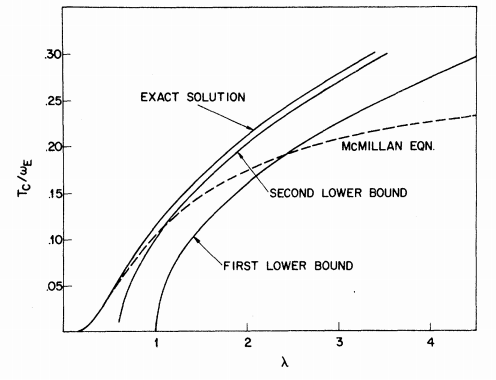
\includegraphics[scale=0.39]{./figures/Tc_theory_dynes.png}
\end{column}
\begin{column}{0.36\textwidth}
\begin{block}{}
Larger $\lambda\Rightarrow$ Larger $T_c/\omega_E$ \\
Larger $\omega_E\Rightarrow$ Larger $T_c$
\end{block}
\end{column}\end{columns}
\end{frame}
%%%%%%%%%%%%%%%%%%%%%%%%%%%%%%%%%%%%%%%%%%%%%%%%%%%%%%%%%%%%%%%%%%%%%%%%%%%%%%%%%%%%%%%%%%%%%%%%%%%%%%%%%%%%%%%%%%%%%%%%%%%%
%%%%%%%%%%%%%%%%%%%%%%%%%%%%%%%%%%%%%%%%%%%%%%%%%%%%%%%%%%%%%%%%%%%%%%%%%%%%%%%%%%%%%%%%%%%%%%%%%%%%%%%%%%%%%%%%%%%%%%%%%%%%
%%%%%%%%%%%%%%%%%%%%%%%%%%%%%%%%%%%%%%%%%%%%%%%%%%%%%%%%%%%%%%%%%%%%%%%%%%%%%%%%%%%%%%%%%%%%%%%%%%%%%%%%%%%%%%%%%%%%%%%%%%%%
\begin{frame}
\frametitle{$T_c$ CALCULATION PHONONS}
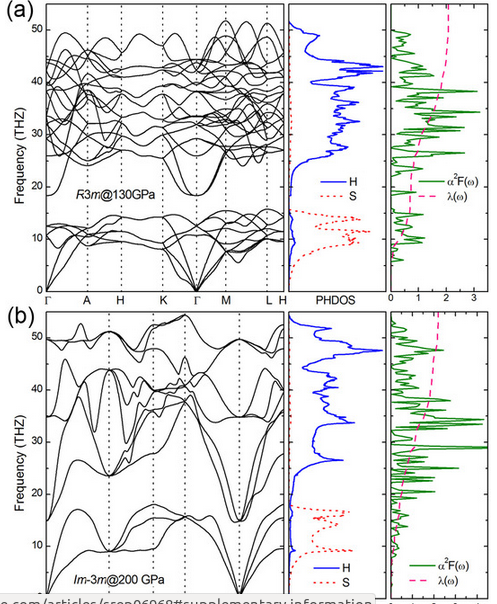
\includegraphics[scale=0.29]{./figures/phonons_duan.png}{\tiny Duan}
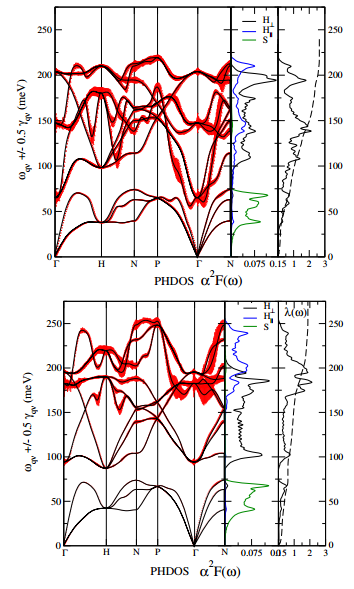
\includegraphics[scale=0.29]{./figures/phonons_errea.png}{\tiny Errea, PRL 114 (2015)}\\
\begin{columns}\begin{column}{0.7\textwidth}
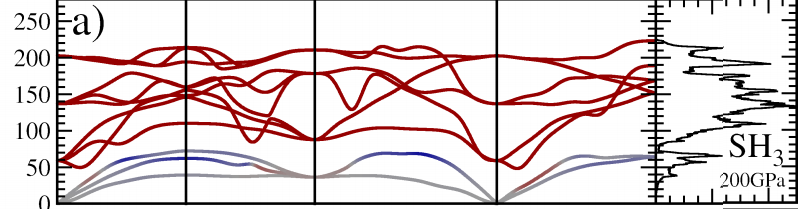
\includegraphics[scale=0.29]{./figures/phonons_flores.png}
\end{column}
\begin{column}{0.36\textwidth}
{\tiny Flores }\\
meV scale, ($\Gamma,N,H,\Gamma,P$), $\alpha^2 F$
\end{column}\end{columns}
\end{frame}
%%%%%%%%%%%%%%%%%%%%%%%%%%%%%%%%%%%%%%%%%%%%%%%%%%%%%%%%%%%%%%%%%%%%%%%%%%%%%%%%%%%%%%%%%%%%%%%%%%%%%%%%%%%%%%%%%%%%%%%%%%%%
%%%%%%%%%%%%%%%%%%%%%%%%%%%%%%%%%%%%%%%%%%%%%%%%%%%%%%%%%%%%%%%%%%%%%%%%%%%%%%%%%%%%%%%%%%%%%%%%%%%%%%%%%%%%%%%%%%%%%%%%%%%%
%%%%%%%%%%%%%%%%%%%%%%%%%%%%%%%%%%%%%%%%%%%%%%%%%%%%%%%%%%%%%%%%%%%%%%%%%%%%%%%%%%%%%%%%%%%%%%%%%%%%%%%%%%%%%%%%%%%%%%%%%%%%
\begin{frame}
\frametitle{$T_c$ CALCULATION PHONONS REVISITED}
$\Delta(\omega_n)Z = -2T\sum\limits_{m}\int d\xi d\omega \frac{\alpha^2(\omega) F(\omega)}{\omega} D(\omega,\omega_n-\omega_m) \frac{\Delta(\omega_m)}{\omega_m^2 + \xi^2}$ \\
$D(\omega,\omega_n-\omega_m) = -\frac{\omega}{[(\omega_n-\omega_m)^2+\omega^2]}$ Phonon Propagator \\
$Z\approx 1+ \lambda$ from renormalized mass\\[1cm]
\begin{block}{McMillan-Dynes-Allen}
-Used by Duan, Flores, Errea \\
-replace $\omega$ in $D$ with average $\tilde{\omega}_E$ \\
-ok for \emph{single low frequency} phonon contribution $\lambda_E$
\end{block}

\begin{block}{Proposed by Gorkov}
-replace $\omega$ in $D$ with average $\tilde{\omega}_{low}$ and $\tilde{\omega}_{high}$ \\
-separate high and low frequency contributions $\lambda_{low}$, $\lambda_{high}$ \\
$\lambda_{low}<\lambda_{high}$
\end{block}
\end{frame}
%%%%%%%%%%%%%%%%%%%%%%%%%%%%%%%%%%%%%%%%%%%%%%%%%%%%%%%%%%%%%%%%%%%%%%%%%%%%%%%%%%%%%%%%%%%%%%%%%%%%%%%%%%%%%%%%%%%%%%%%%%%%
%%%%%%%%%%%%%%%%%%%%%%%%%%%%%%%%%%%%%%%%%%%%%%%%%%%%%%%%%%%%%%%%%%%%%%%%%%%%%%%%%%%%%%%%%%%%%%%%%%%%%%%%%%%%%%%%%%%%%%%%%%%%
%%%%%%%%%%%%%%%%%%%%%%%%%%%%%%%%%%%%%%%%%%%%%%%%%%%%%%%%%%%%%%%%%%%%%%%%%%%%%%%%%%%%%%%%%%%%%%%%%%%%%%%%%%%%%%%%%%%%%%%%%%%%
\begin{frame}
\frametitle{ELECTRON BANDS}
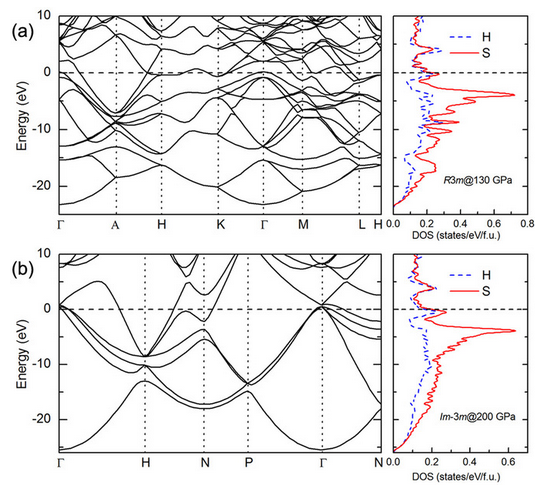
\includegraphics[scale=0.29]{./figures/electrons_duan.png}
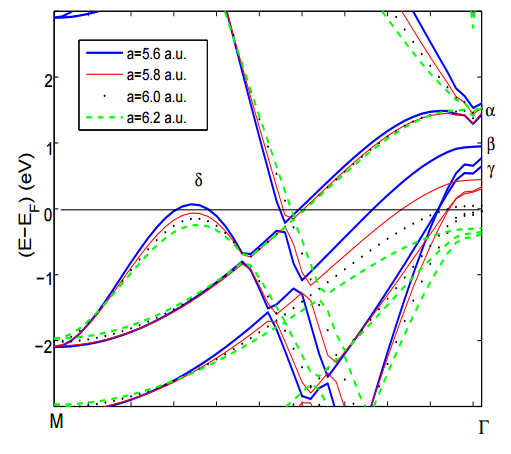
\includegraphics[scale=0.29]{./figures/electrons_bianconi.png}\\
\centering Duan, Bianconi\\[0.2cm]
Hole pockets form in Im-3m phase with pressure \\
\begin{block}{Gorkov}
$T_c$ decrease for $P>150GPa$ due to hole pocket coupling to high frequency phonons??
\end{block}

\end{frame}
%%%%%%%%%%%%%%%%%%%%%%%%%%%%%%%%%%%%%%%%%%%%%%%%%%%%%%%%%%%%%%%%%%%%%%%%%%%%%%%%%%%%%%%%%%%%%%%%%%%%%%%%%%%%%%%%%%%%%%%%%%%%
%%%%%%%%%%%%%%%%%%%%%%%%%%%%%%%%%%%%%%%%%%%%%%%%%%%%%%%%%%%%%%%%%%%%%%%%%%%%%%%%%%%%%%%%%%%%%%%%%%%%%%%%%%%%%%%%%%%%%%%%%%%%
%%%%%%%%%%%%%%%%%%%%%%%%%%%%%%%%%%%%%%%%%%%%%%%%%%%%%%%%%%%%%%%%%%%%%%%%%%%%%%%%%%%%%%%%%%%%%%%%%%%%%%%%%%%%%%%%%%%%%%%%%%%%
\begin{frame}
\frametitle{ANOMALOUS ISOTOPE EFFECT}
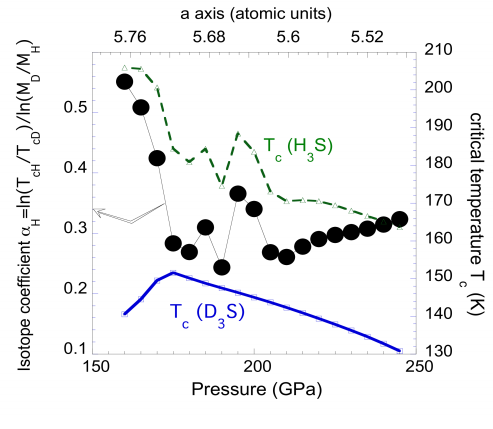
\includegraphics[scale=0.29]{./figures/anomalous_isotope_bianconi.png}\quad
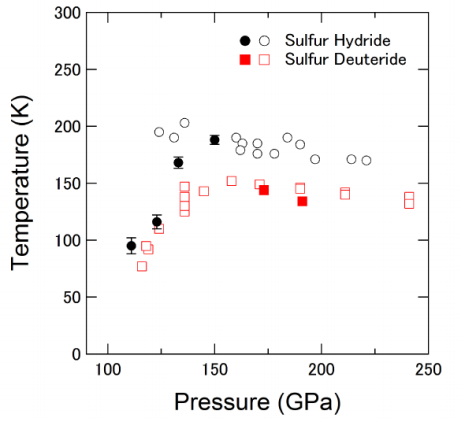
\includegraphics[scale=0.3]{./figures/PT_einaga.png} \\
Bianconi, Einaga \\[0.3cm]
\begin{block}{Gorkov}
Possibly explained by $\lambda_{low}\approx\lambda_{high}$ in R3m phase and $\lambda_{low}<\lambda_{high}$
\end{block}.
\end{frame}
%%%%%%%%%%%%%%%%%%%%%%%%%%%%%%%%%%%%%%%%%%%%%%%%%%%%%%%%%%%%%%%%%%%%%%%%%%%%%%%%%%%%%%%%%%%%%%%%%%%%%%%%%%%%%%%%%%%%%%%%%%%%
%%%%%%%%%%%%%%%%%%%%%%%%%%%%%%%%%%%%%%%%%%%%%%%%%%%%%%%%%%%%%%%%%%%%%%%%%%%%%%%%%%%%%%%%%%%%%%%%%%%%%%%%%%%%%%%%%%%%%%%%%%%%
%%%%%%%%%%%%%%%%%%%%%%%%%%%%%%%%%%%%%%%%%%%%%%%%%%%%%%%%%%%%%%%%%%%%%%%%%%%%%%%%%%%%%%%%%%%%%%%%%%%%%%%%%%%%%%%%%%%%%%%%%%%%
\begin{frame}
\frametitle{END}
QUESTIONS???
\end{frame}
\bibliography{/home/ben/School/MyBib/mybib}
\end{document}